\section{Exercise 3}
\subsection*{3.1}
\begin{figure}[H]
	\centering
	\begin{subfigure}[b]{0.42\linewidth}
		\centering
		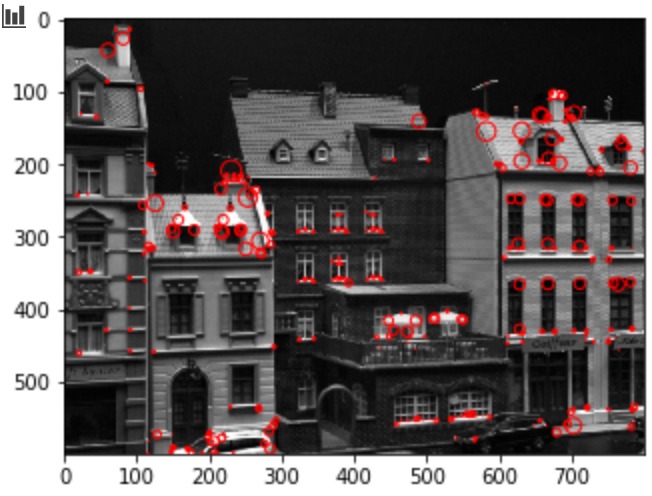
\includegraphics[width=\linewidth]{Materials/E3/k1a005}
		\caption{$k = 1$, $\alpha = 0.05$.}
	\end{subfigure}
	\hfill
	\begin{subfigure}[b]{0.42\linewidth}
		\centering
		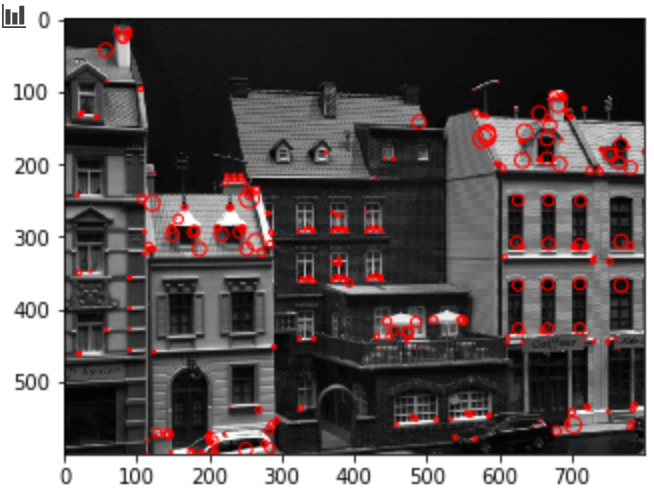
\includegraphics[width=\linewidth]{Materials/E3/k1a015}
		\caption{$k = 1$, $\alpha = 0.15$.}
	\end{subfigure}
	\\
	\begin{subfigure}[b]{0.42\linewidth}
		\centering
		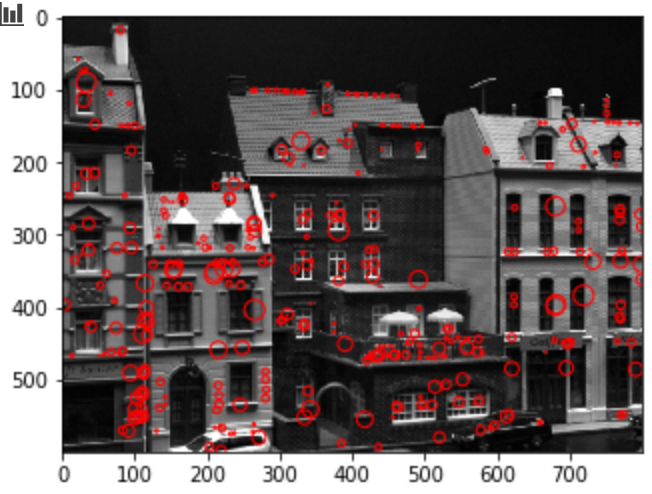
\includegraphics[width=\linewidth]{Materials/E3/k1a095}
		\caption{$k = 1$, $\alpha = 0.95$.}
	\end{subfigure}
	\hfill
	\begin{subfigure}[b]{0.42\linewidth}
		\centering
		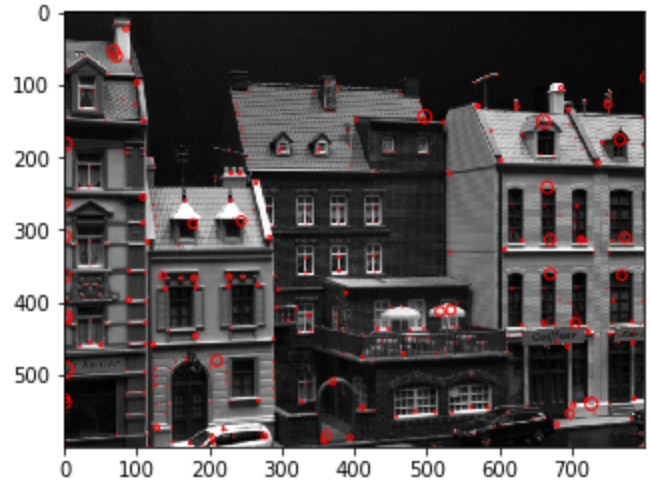
\includegraphics[width=\linewidth]{Materials/E3/k4a005}
		\caption{$k = 2$, $\alpha = 0.15$.}
	\end{subfigure}
	\begin{subfigure}[b]{0.42\linewidth}
		\centering
		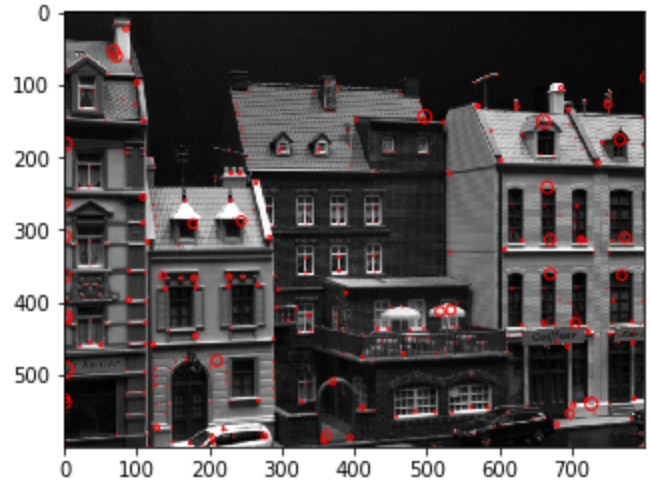
\includegraphics[width=\linewidth]{Materials/E3/k4a005}
		\caption{$k = 4$, $\alpha = 0.05$.}
	\end{subfigure}
	\hfill
	\begin{subfigure}[b]{0.42\linewidth}
		\centering
		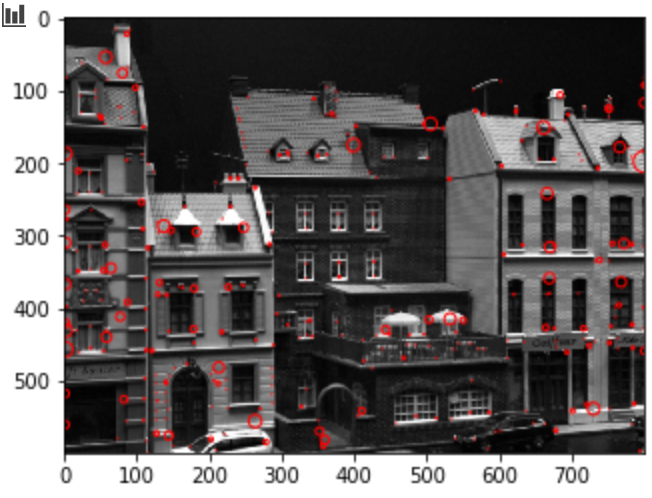
\includegraphics[width=\linewidth]{Materials/E3/k4a015}
		\caption{$k = 4$, $\alpha = 0.15$.}
	\end{subfigure}
	\\
	\begin{subfigure}[b]{0.4\linewidth}
		\centering
		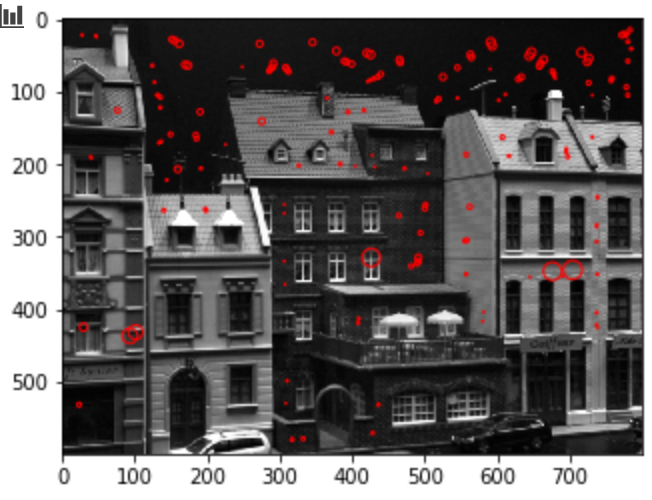
\includegraphics[width=\linewidth]{Materials/E3/k4a095}
		\caption{$k = 4$, $\alpha = 0.95$.}
	\end{subfigure}
	\caption{Multi -scale Harris corner detection with various \textit{k} and $\alpha$ values.}
	\label{corners}
\end{figure}
In \autoref{corners} we see the results of the multi-scale Harris corner detection for various values of \textit{k} and $\alpha$. The range of scales is 30 evenly spaced values between $2^0$ and $2^5$ as advised in the assignment text. In \autoref{E3code} we see the code used for this exercise. We see that if we increase the $\alpha$ value too much we begin to detect edges rather than corners. We also see if increase the combination of \textit{k} and $\alpha$ too much (i.e. the last image) we start to get unusable results. We find the best result to be with \textit{k} around 2 and $\alpha$ around $0.15$.

\begin{figure}[H]
	\centering
	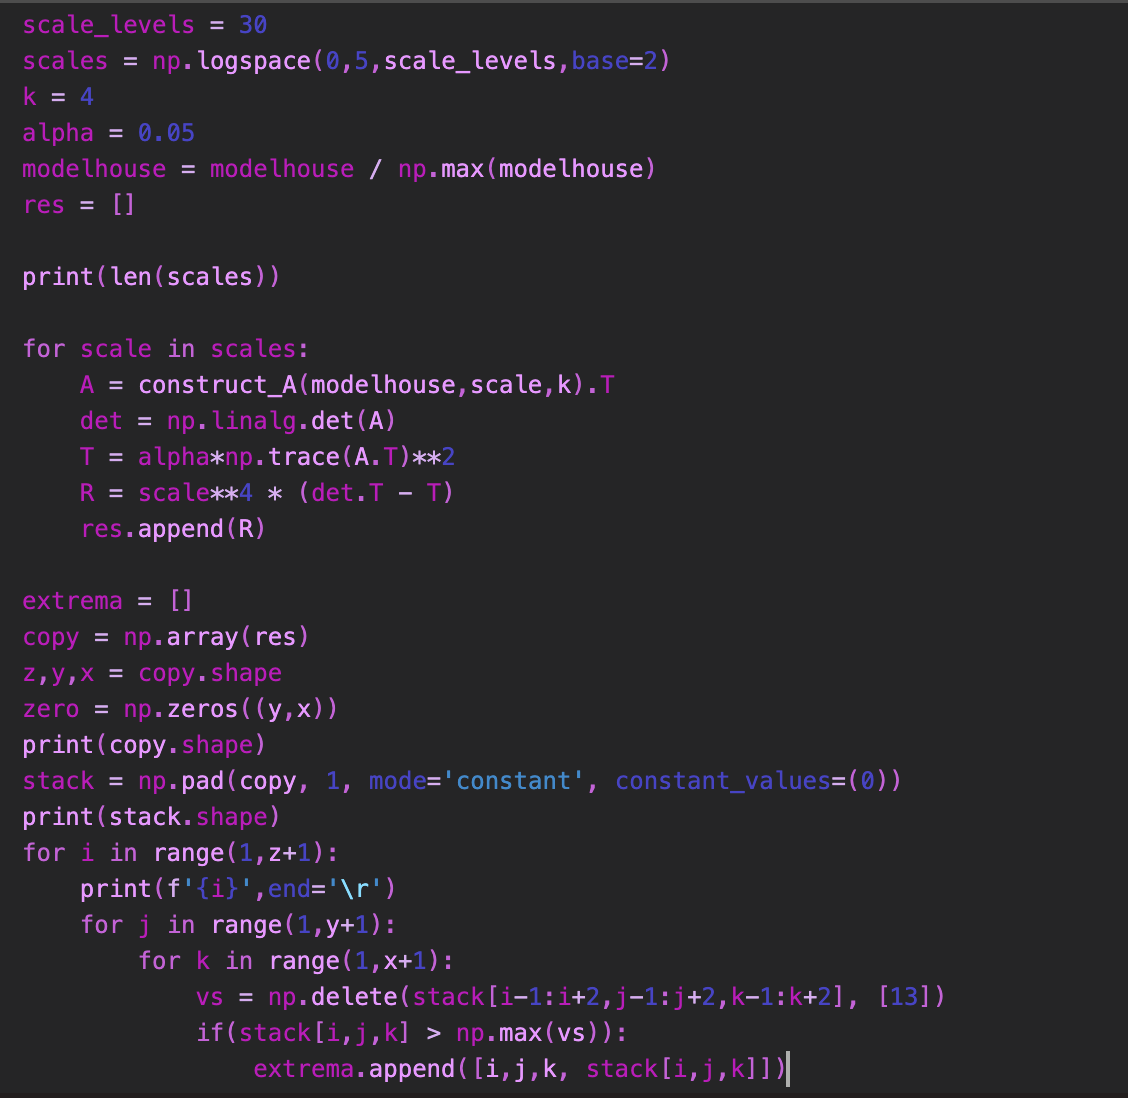
\includegraphics[width=0.8\linewidth]{Materials/E3/code1}
	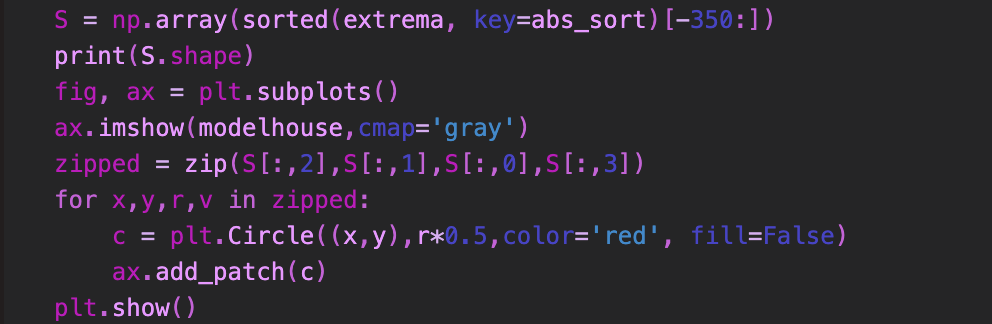
\includegraphics[width=0.8\linewidth]{Materials/E3/code2}
	\caption{Code used for this exercise.}
	\label{E3code}
\end{figure}